%------------------------------------------------------------------------------
% Tema 2. Semiologia
%------------------------------------------------------------------------------
\section{Semiologia}

\subsection{Valors de refer�ncia}
La poblaci� de refer�ncia �s la poblaci� individus sans (normals). Per estudiar-ho, s'agafa una mostra de refer�ncia, que �s un nombre assequible i representatiu de la poblaci� de refer�ncia.

\begin{description}
\item[Valors de refer�ncia] Rang de resultat anal�tic de la determinaci� d'un par�metre bioqu�mic en esp�cimens d'individus de refer�ncia.

\item[Capacitat discriminant] Propietat de donar valors diferents en individus d'una poblaci� normal ($\hat{E}$) respecte els d'una poblaci� patol�gica ($E$).
\end{description}

\subsection{Determinaci� de la capacitat discriminant}
La capacitat discriminant es mesura amb:
\begin{itemize}
\item \textbf{Sensibilitat:} Probabilitat d'obtenir un resultat positiu en un
  individu de E (malalt).
  \begin{equation}
    \label{eq:1}
    \frac{PC}{PC+NF}
  \end{equation}
On $PC$ s�n els positius certs i $NF$ els negatius falsos. Seria el nombre de malalts detectats entre els malalts totals.

\item \textbf{Especificitat:} Probabilitat d'obtenir un resultat
  negatiu en un individu de $\hat{E}$ (encertar amb un sa).
  \begin{equation}
    \label{eq:2}
    \frac{NC}{NC+PF}
  \end{equation}

On $NC$ s�n els negatius certs i $PF$ els positius falsos. Seria el
nombre de sans detectats entre els sans totals.

\item \textbf{Efic�cia diagn�stica} �s el quocient d'individus
  classificats correctament en la poblaci� de malalts ($E$) o de sans
  ($\hat{E}$) respecte el total de la mostra:
  \begin{equation}
    \label{eq:3}
    \frac{PC+NC}{PC+NF+NC+PF}
  \end{equation}

\item \textbf{Valor predictiu} �s la probabilitat de patir la malaltia
  quan el resultat e??s positiu i de no patir-la quan el resultat e??s
  negatiu.
  \begin{itemize}
  \item Positiu: Probabilitat de patir-la si el diagno??stic �s positiu:
    \begin{equation}
      \label{eq:4}
      \frac{PC}{PC+NF}
    \end{equation}
  \item Negatiu: Probabilitat de patir-la si el diagno??stic �s negatiu:
    \begin{equation}
      \label{eq:5}
      \frac{NC}{NC+NF}
    \end{equation}
  \end{itemize}
\end{itemize}

\subsubsection*{Exemple}
\begin{figure}[H]
  \centering
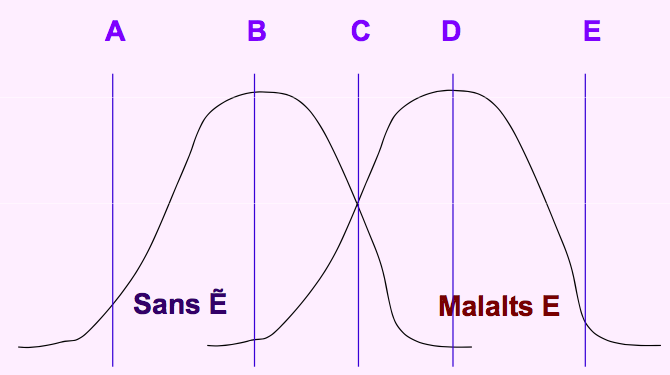
\includegraphics[width=0.9\textwidth]{fig1}  
\end{figure}

\begin{itemize}
\item En A la sensibilitat e??s ma??xima (1) i l???especificitat e??s mi??nima
  (0)
\item En B la sensibilitat �s m�xima (0.95) i l'especificitat �s 0.5.
\item En C la sensibilitat �s 0.76 i l'especificitat �s 0.75.
\item En D la sensibilitat �s 0.5 i l'especificitat �s 0.95.
\item En E la sensibilitat e??s mi??nima (0) i l???especificitat e??s ma??xima (1)
\end{itemize}